\documentclass{article}
\usepackage{amsmath, amssymb, amsfonts, amsthm}
\usepackage{tikz}

\begin{document}

\begin{figure}[h]
    \centering
    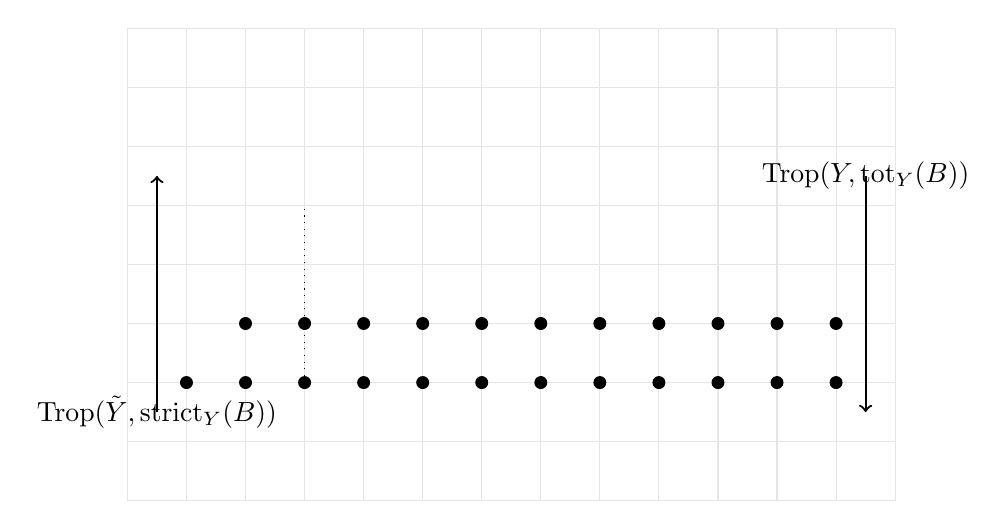
\begin{tikzpicture}[scale=0.75]
        % Draw the grid
        \draw[step=1cm, gray!20] (-3,-2) grid (10,6);
        
        % Draw filled circles
        \filldraw[black] (-2, 0) circle (0.1);
        \filldraw[black] (-1, 0) circle (0.1);
        \filldraw[black] (0, 0) circle (0.1);
        \filldraw[black] (1, 0) circle (0.1);
        \filldraw[black] (2, 0) circle (0.1);
        \filldraw[black] (3, 0) circle (0.1);
        \filldraw[black] (4, 0) circle (0.1);
        \filldraw[black] (5, 0) circle (0.1);
        \filldraw[black] (6, 0) circle (0.1);
        \filldraw[black] (7, 0) circle (0.1);
        \filldraw[black] (8, 0) circle (0.1);
        \filldraw[black] (9, 0) circle (0.1);
        \filldraw[black] (-1, 1) circle (0.1);
        \filldraw[black] (0, 1) circle (0.1);
        \filldraw[black] (1, 1) circle (0.1);
        \filldraw[black] (2, 1) circle (0.1);
        \filldraw[black] (3, 1) circle (0.1);
        \filldraw[black] (4, 1) circle (0.1);
        \filldraw[black] (5, 1) circle (0.1);
        \filldraw[black] (6, 1) circle (0.1);
        \filldraw[black] (7, 1) circle (0.1);
        \filldraw[black] (8, 1) circle (0.1);
        \filldraw[black] (9, 1) circle (0.1);
        
        % Dotted vertical line
        \draw[dotted] (0, 0) -- (0, 3);
        
        % Draw annotations
        \node at (-2.5, -0.5) {\text{Trop}$(\tilde{Y}, \text{strict}_Y(B))$};
        \node at (9.5, 3.5) {\text{Trop}$(Y, \text{tot}_Y(B))$};
        
        % Draw arrows
        \draw[->,thick] (-2.5, -0.5) -- (-2.5, 3.5);
        \draw[->,thick] (9.5, 3.5) -- (9.5, -0.5);
    \end{tikzpicture}
    \caption*{Graphical summary of $\mathbb{P}(1,1,4)$, Case II. When the integer point $(0,4)$ is missing from $\mathrm{Newt}(\Omega)$, we move the edge corresponding to the exceptional divisor of the minimal resolution $\mathbb{F}_4 \to \mathbb{P}(1,1,4)$ normally inwards until it reaches an integer point. The new edge has affine length $4$, which implies that the strict transform of the branch curve intersects the contracted $-4$-curve $C_1$ with total multiplicity $4$. The affine distance from the missing point to the new edge is $1$, so the curve $C_1$ appears in $\mathrm{tot}_{\tilde{Y}}(B)$ with multiplicity $1$.}
\end{figure}

\end{document}